\documentclass[10pt,a4paper]{article}
\usepackage[margin=0.65in,top=0.6in,bottom=0.6in]{geometry}
\usepackage{graphicx}
\usepackage{booktabs}
\usepackage{amsmath}
\usepackage{hyperref}
\usepackage{float}
\usepackage{caption}
\usepackage{subcaption}
\usepackage[table]{xcolor}
\usepackage{enumitem}
\usepackage{multicol}
\usepackage{titlesec}
\usepackage{array}
\usepackage{setspace}

\graphicspath{{../figures/}}

\captionsetup{font=small,skip=3pt}
\setlength{\parskip}{2pt}
\setlength{\parindent}{0pt}
\setlength{\columnsep}{0.25in}
\titlespacing*{\section}{0pt}{6pt}{3pt}
\titlespacing*{\subsection}{0pt}{4pt}{2pt}
\titleformat{\section}{\normalsize\bfseries}{\thesection.}{0.4em}{}
\titleformat{\subsection}{\small\bfseries}{\thesubsection}{0.4em}{}
\setlist{nosep,leftmargin=1.2em}
\setstretch{0.95}

\pagestyle{empty}

\begin{document}

% ── Title ─────────────────────────────────────────────────
\begin{center}
{\large\bfseries Media vs.\ Public Opinion on GLP-1 Weight-Loss Drugs}\\[2pt]
{\small A Comparative Text-Analytics Study of Ozempic \& Wegovy}\\[2pt]
{\footnotesize Vasilis Christopoulos, Hugo Guideau, Saksi Khosla, Mustafa Yousuf, Othmane Zizi\\
INSY 669 -- Text Analytics $\mid$ McGill University $\mid$ Winter 2026}
\end{center}
\vspace{-2pt}
\hrule
\vspace{4pt}

\begin{multicols}{2}

\section{Introduction}

GLP-1 receptor agonists---Ozempic and Wegovy---have sparked extensive online patient discussion and media coverage.  This study compares \textbf{public discourse} (3,246~Reddit posts + 102~WebMD reviews) with \textbf{media discourse} (634~Google News articles) from January--November~2024, asking: (1)~How does sentiment differ? (2)~What linguistic and thematic gaps exist? (3)~Does either stream lead the other temporally?

\section{Data \& Methodology}

\begin{table}[H]
\centering\small
\begin{tabular}{llrl}
\toprule
\textbf{Source} & \textbf{Type} & $n$ & \textbf{Method}\\
\midrule
Reddit & Public & 3,246 & Arctic Shift API\\
WebMD & Public & 102 & Web scraping\\
Google News & Media & 634 & RSS + URL decode\\
\bottomrule
\end{tabular}
\end{table}
\vspace{-6pt}

We used a \textbf{hybrid} media-text strategy (full article body when available, snippet fallback otherwise).  Preprocessing included tokenisation, stopword removal, and lemmatisation.  A \textbf{length-normalised track} (first 40~tokens) controls for document-length confounds.  All ML pipelines use stratified $k$-fold CV to prevent leakage.

\section{Results}

\subsection{Sentiment Analysis}

VADER scores reveal a significant gap: public mean $= +0.121$, media $= -0.137$ ($t = 9.43$, $p < 0.001$, Cohen's $d = 0.44$).  Reddit is moderately positive ($+0.135$), WebMD strongly negative ($-0.308$), and news negative ($-0.137$).  All pairwise Mann--Whitney $U$ tests are significant ($p < 0.001$).

\begin{figure}[H]
\centering
\begin{subfigure}[t]{0.48\linewidth}
  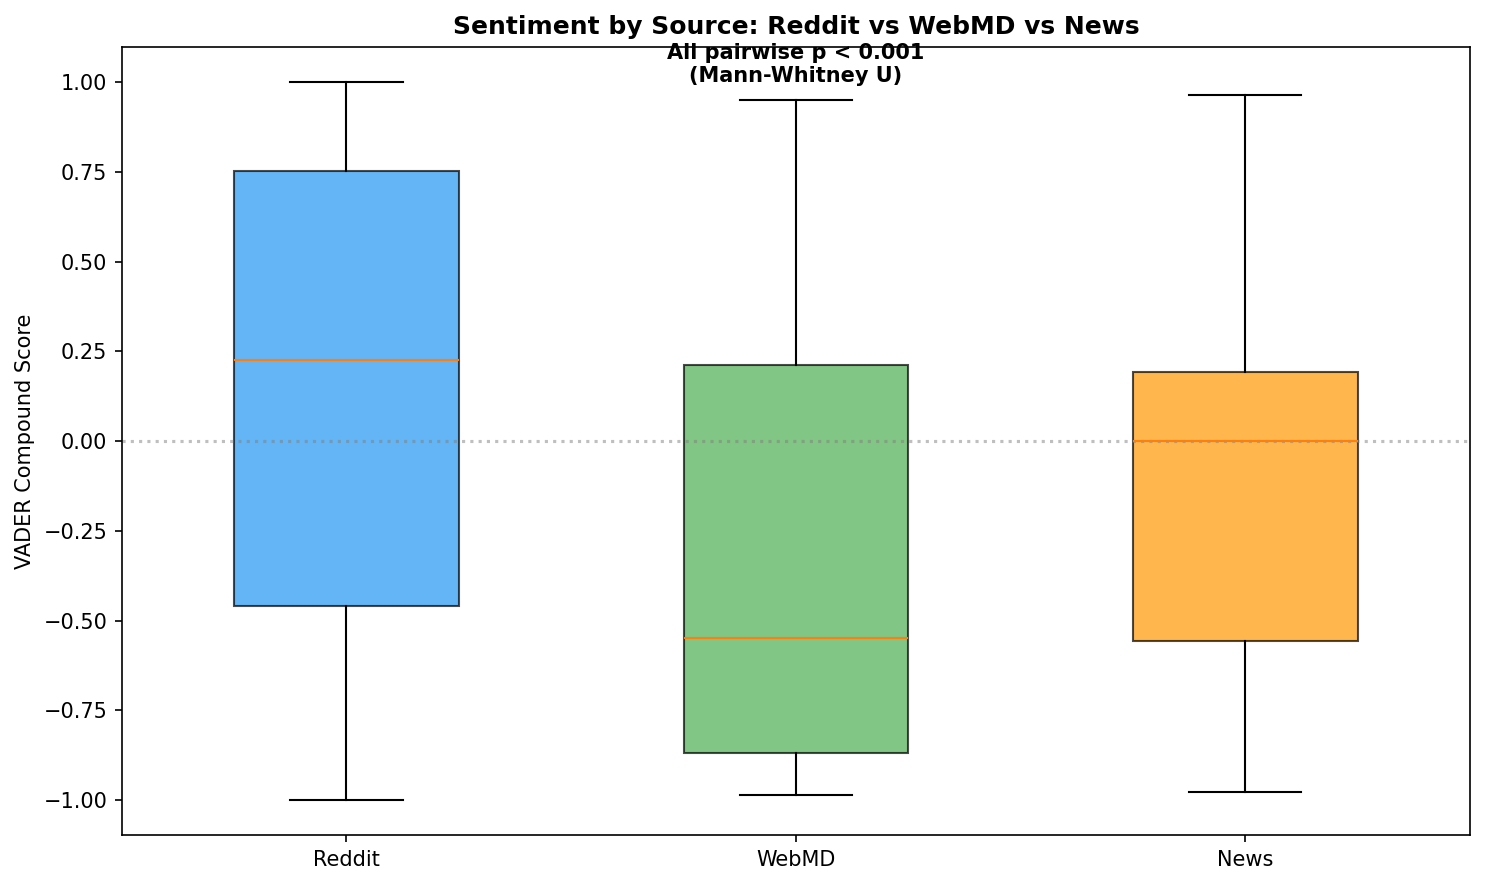
\includegraphics[width=\linewidth]{sentiment_boxplot_3source.png}
\end{subfigure}
\hfill
\begin{subfigure}[t]{0.48\linewidth}
  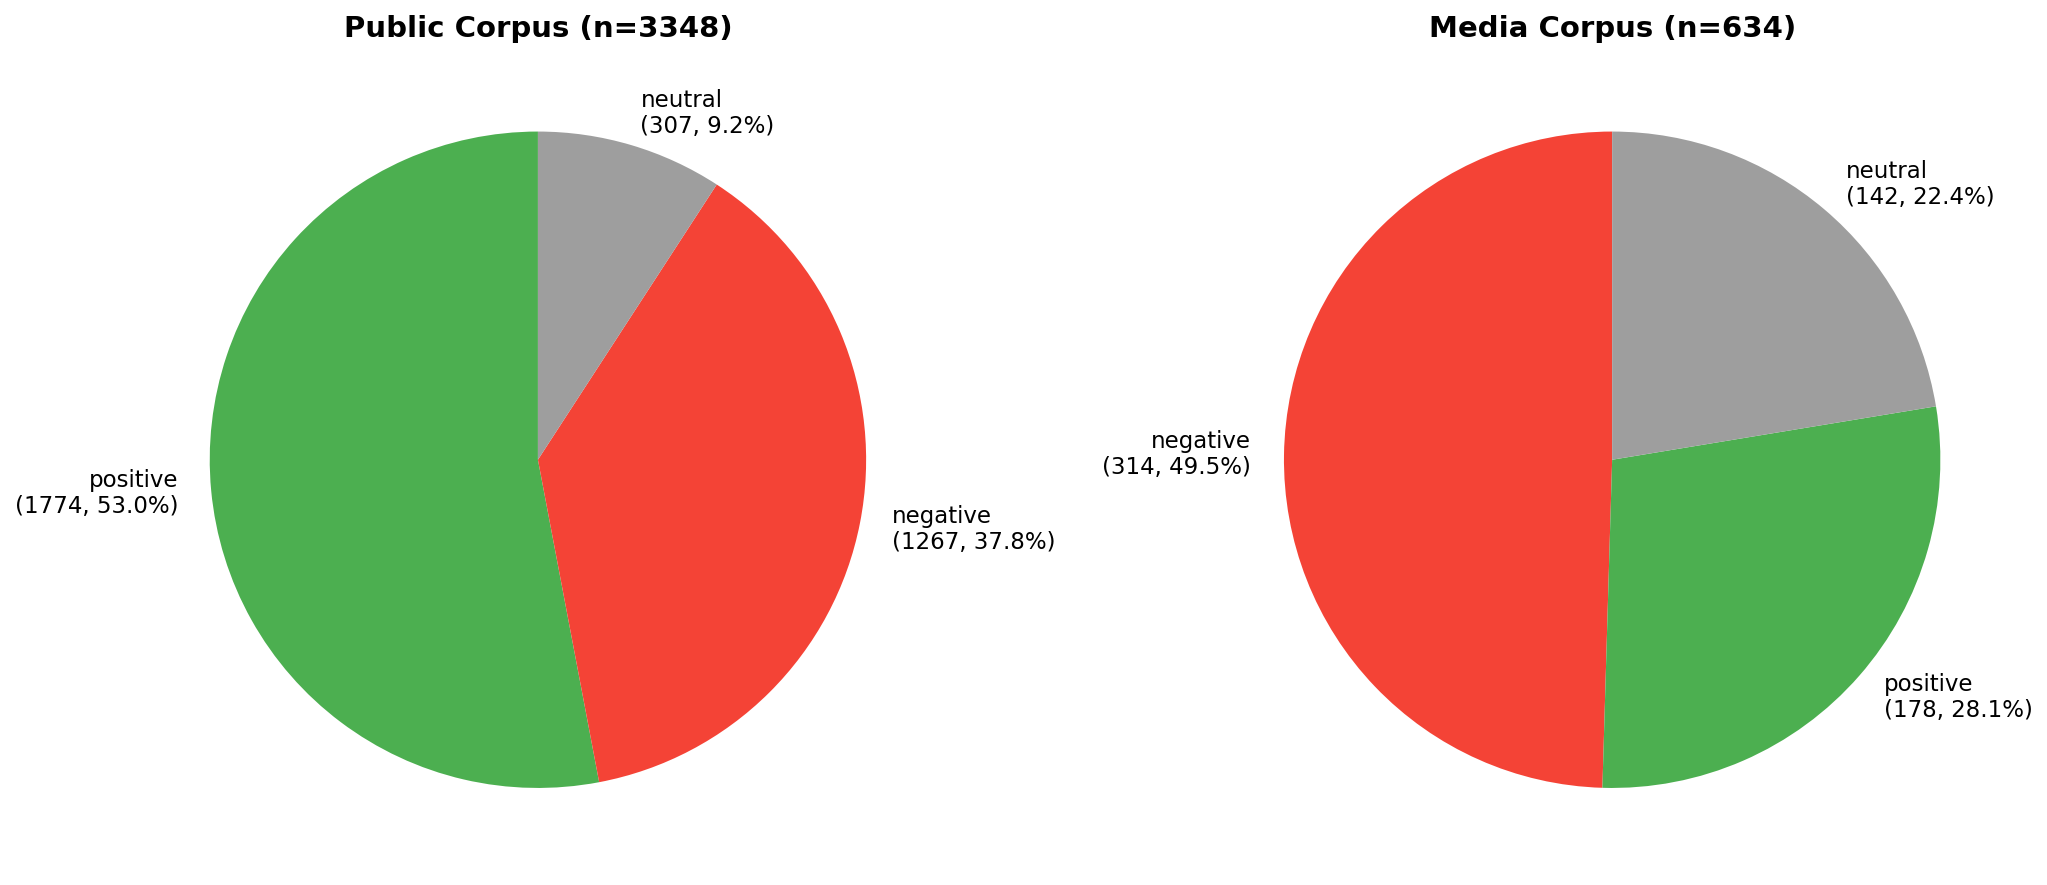
\includegraphics[width=\linewidth]{sentiment_pies.png}
\end{subfigure}
\vspace{-4pt}
\caption{Sentiment by source and label distribution.}
\end{figure}

\subsection{Corpus Comparison \& Side Effects}

TF-IDF top terms confirm thematic divergence: public emphasises \emph{week, dose, lb, anyone}; media foregrounds \emph{semaglutide, drug, weightloss drug}.  Cosine similarity between mean vectors: 0.346 (0.350 normalised).

A targeted side-effect analysis shows public mentions nausea (3.38/1k tokens), diarrhea (1.22), constipation (1.16), and anxiety (0.69) at rates far exceeding media, where most side effects have zero mentions.  Gaps persist under normalisation.

\begin{figure}[H]
\centering
\begin{subfigure}[t]{0.48\linewidth}
  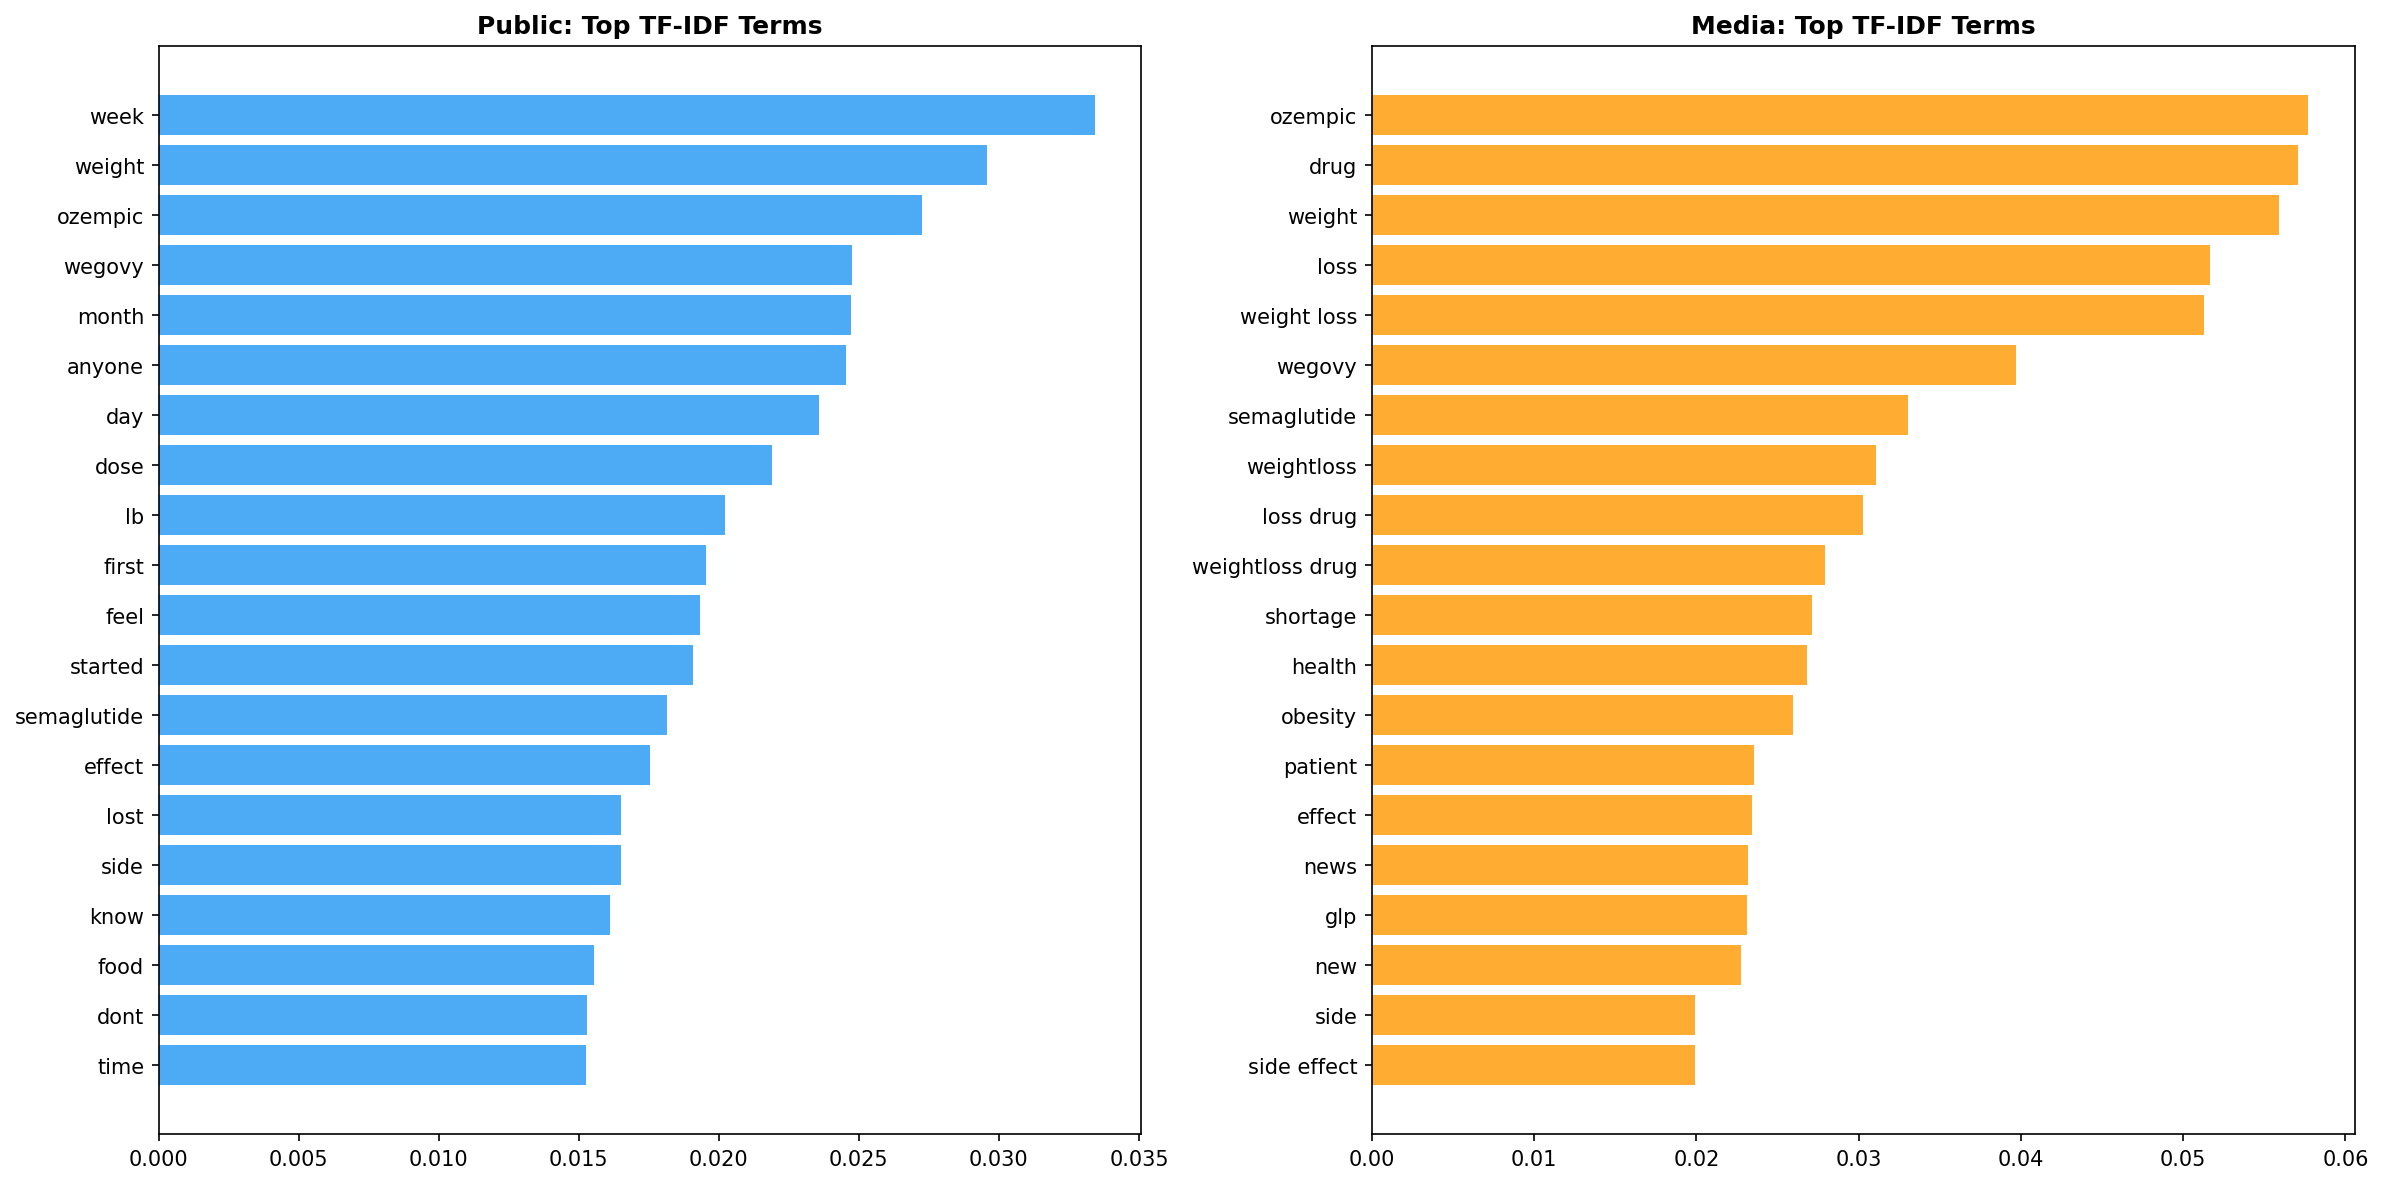
\includegraphics[width=\linewidth]{tfidf_comparison.png}
\end{subfigure}
\hfill
\begin{subfigure}[t]{0.48\linewidth}
  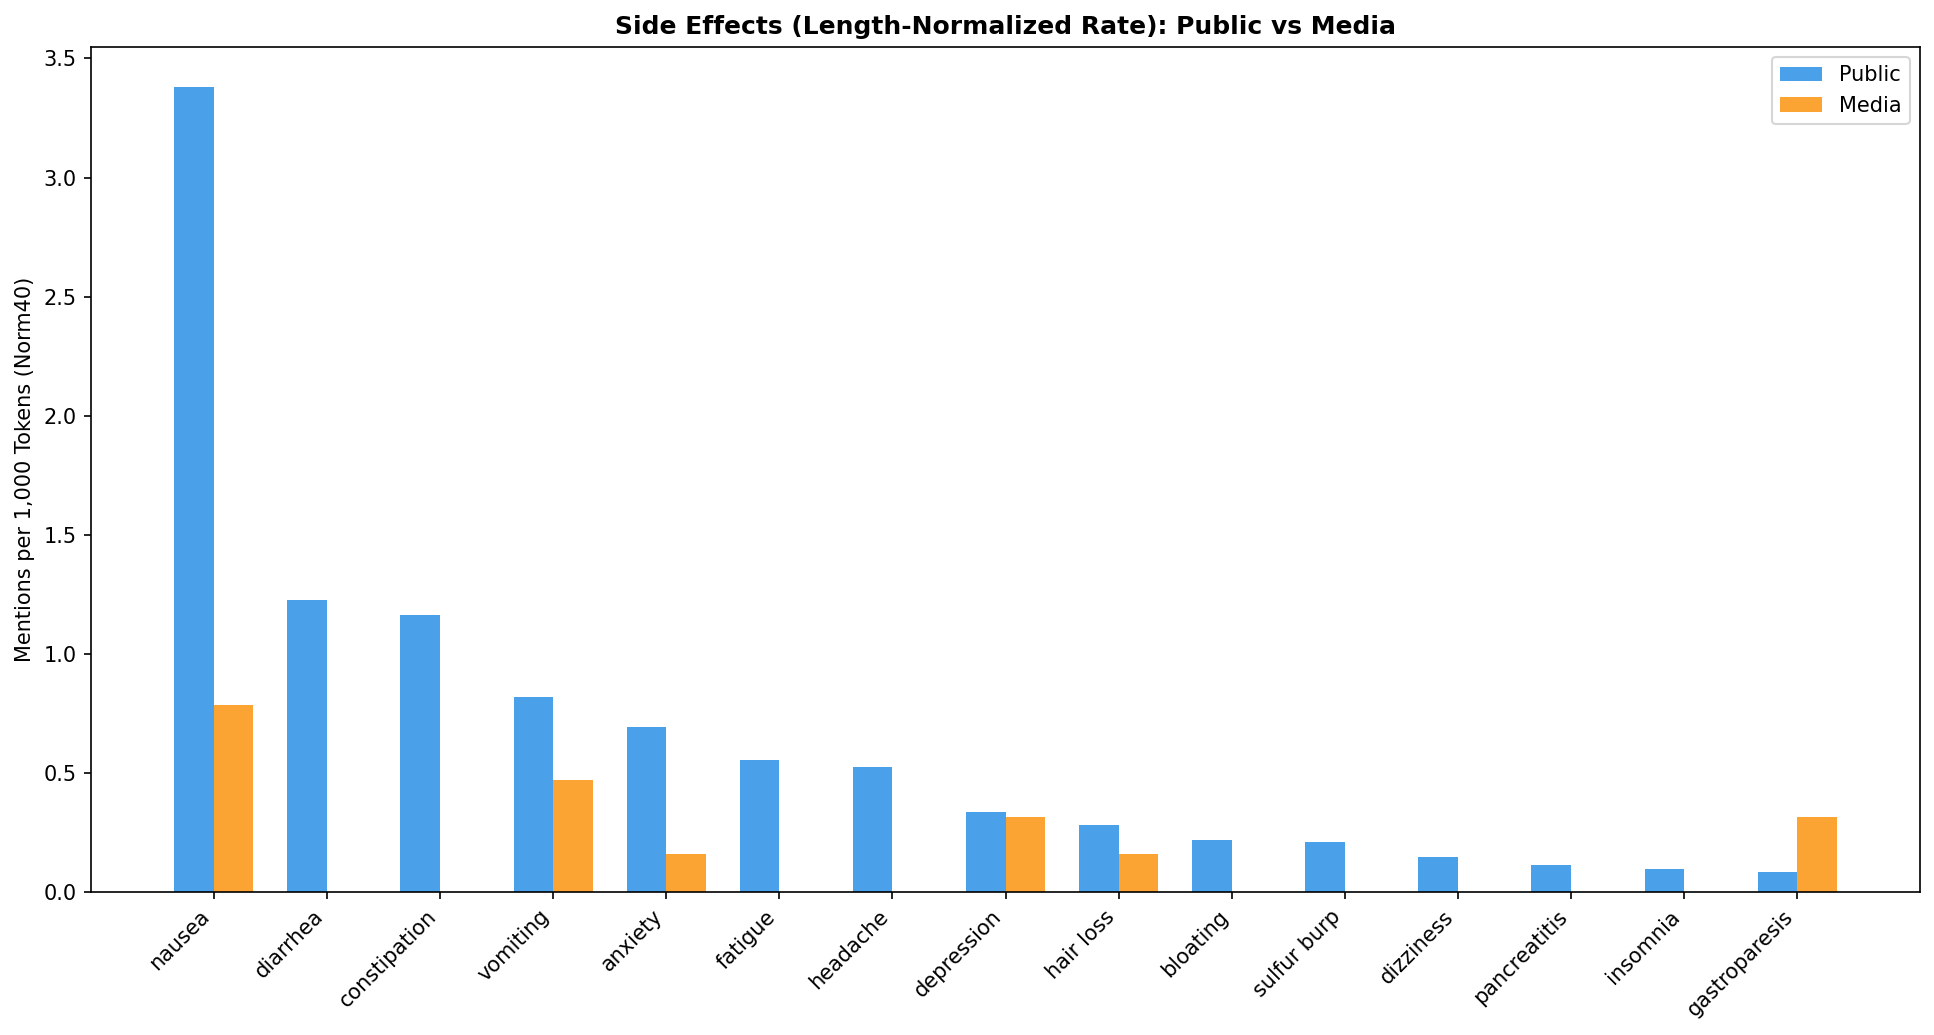
\includegraphics[width=\linewidth]{side_effects_normalized_rate.png}
\end{subfigure}
\vspace{-4pt}
\caption{TF-IDF comparison (left) and side-effect rates per 1k tokens (right).}
\end{figure}

\subsection{Classification}

Na\"ive Bayes ($\alpha{=}0.1$): \textbf{97.6\%} CV accuracy.  KNN ($k{=}7$): \textbf{96.7\%}.  Normalised-track accuracy is nearly identical (97.6\% / 96.4\%), confirming separability is vocabulary-driven, not length-driven.  Top public features: \emph{anyone, day, lb, feeling}; top media: \emph{cnn, healthline, medscape, nbc}.

\subsection{Topic Modelling}

LDA (5~topics/corpus) reveals public topics centred on dosing, insurance, weight progress, and compounding; media topics on clinical trials, FDA regulation, and Medicare access.  $K$-means ($k{=}2$) purity: \textbf{84.1\%}---strong unsupervised separation.

\subsection{Aspect-Based Sentiment}

Sentiment was computed across seven aspects.  The largest discrepancies:

\begin{table}[H]
\centering\small
\begin{tabular}{lrrrl}
\toprule
\textbf{Aspect} & \textbf{Pub.} & \textbf{Med.} & \textbf{Gap} & \textbf{Sig.}\\
\midrule
Mental health & $-0.10$ & $-0.74$ & 0.63 & $p{=}.040$*\\
Access & $+0.20$ & $-0.35$ & 0.55 & $p{<}.001$*\\
Efficacy & $+0.14$ & $-0.33$ & 0.46 & $p{<}.001$*\\
Cost & $+0.16$ & $-0.02$ & 0.18 & $p{=}.017$*\\
Side effects & $-0.03$ & $-0.20$ & 0.16 & $p{=}.666$\\
\bottomrule
\end{tabular}
\end{table}
\vspace{-4pt}

Media is dramatically more negative on mental health ($-0.74$ vs.\ $-0.10$), likely driven by alarming headlines.  A discrepancy logistic-regression classifier achieves 83.7\% accuracy.

\subsection{Temporal Lead-Lag}

Granger causality tests (max lag~4 weeks, 45~observations) find no significant relationship in either direction (Media$\to$Public $p{=}0.37$; Public$\to$Media $p{=}0.30$).  Cross-correlation peaks at lag~$-7$ weeks ($r{=}0.31$).  The two streams appear to respond to shared events rather than driving each other.

\begin{figure}[H]
\centering
\begin{subfigure}[t]{0.48\linewidth}
  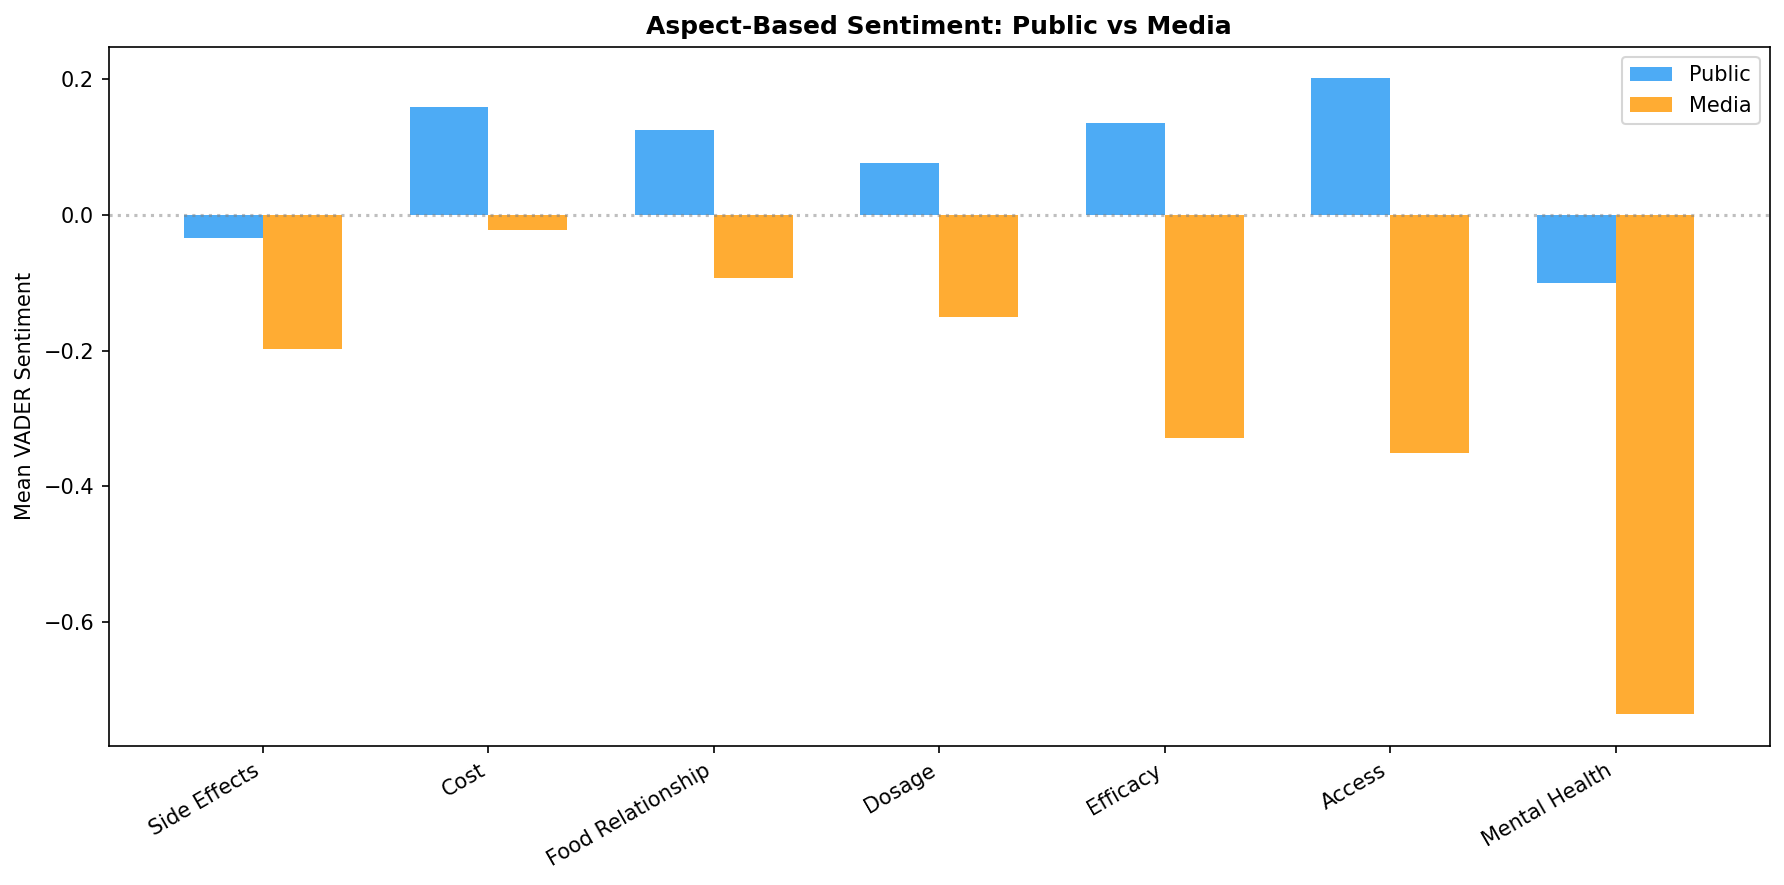
\includegraphics[width=\linewidth]{aspect_sentiment_comparison.png}
\end{subfigure}
\hfill
\begin{subfigure}[t]{0.48\linewidth}
  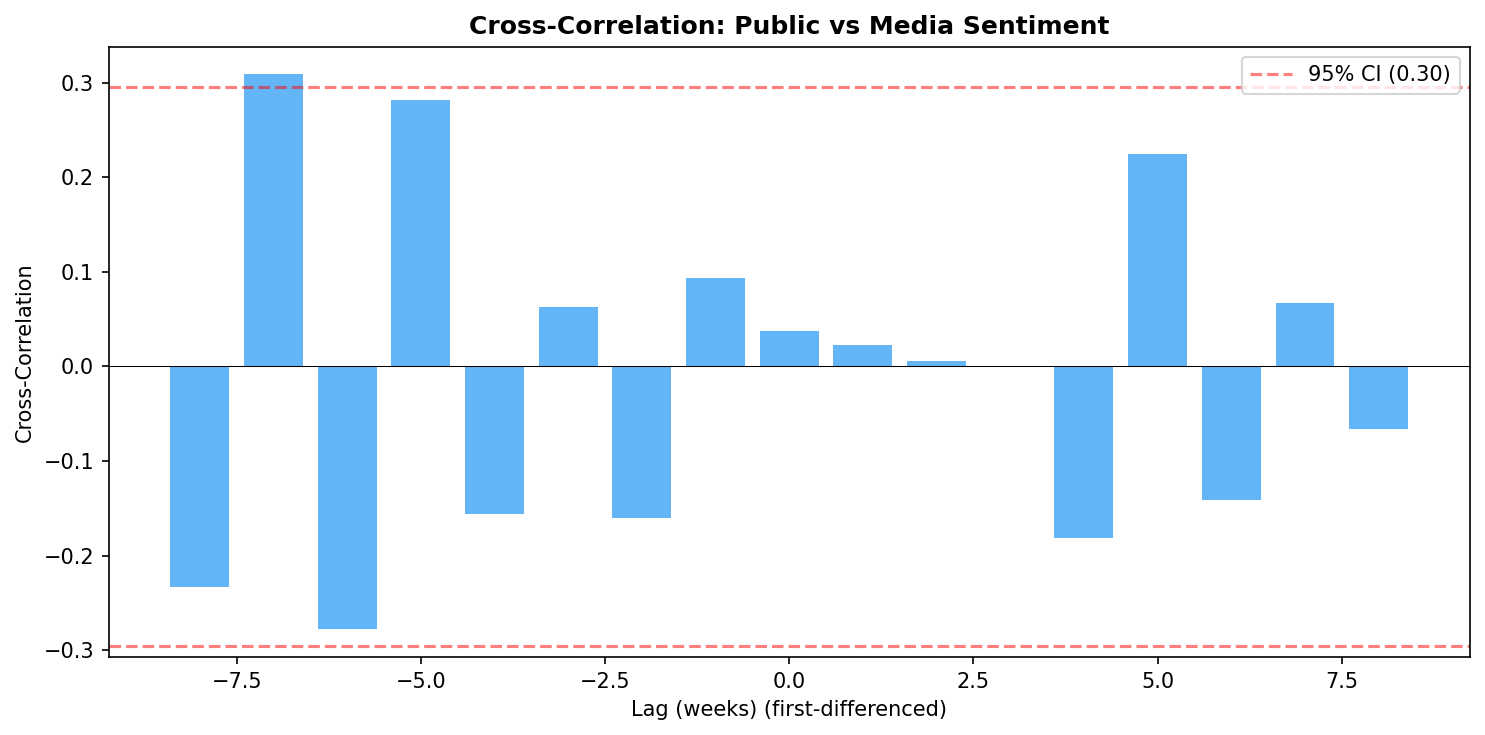
\includegraphics[width=\linewidth]{crosscorrelation.png}
\end{subfigure}
\vspace{-4pt}
\caption{Aspect sentiment (left) and cross-correlation (right).}
\end{figure}

\section{Discussion}

The sentiment gap aligns with prior health-communication research: media defaults to cautionary framing while patients share mixed lived experiences.  WebMD's strong negativity ($-0.31$) suggests review-selection bias.  The 97.6\% classification accuracy---stable under normalisation---confirms fundamentally different registers.

The side-effect coverage gap has real-world implications: patients relying on media may underestimate everyday symptom burden (nausea, constipation, anxiety), while providers could monitor patient communities for emerging signals absent from news.  The mental-health aspect discrepancy is particularly striking: media amplifies alarm while patients report only mild negativity.

\textbf{Limitations.}  Hybrid mode used 100\% snippet fallback (no pre-extracted bodies); VADER may miss medical-domain nuance; 45 weekly observations limit Granger power; Reddit/WebMD are not representative of all patients.

\section{Conclusion}

Public and media discourse on GLP-1 drugs diverge significantly in sentiment, vocabulary, and thematic emphasis.  These differences are robust across analytical methods and length normalisation.  Patients relying solely on media may form an incomplete picture; healthcare providers should monitor both streams.

\vspace{4pt}
{\footnotesize\textbf{Reproducibility.} \texttt{python project\_cli.py run-analysis --media-text-mode hybrid}}

\end{multicols}
\end{document}
